\documentclass[12pt]{scrartcl}



\setlength{\parindent}{0pt}
\setlength{\parskip}{.25cm}

\usepackage{graphicx}

\usepackage{xcolor}

\definecolor{darkred}{rgb}{0.5,0,0}
\definecolor{darkgreen}{rgb}{0,0.5,0}
\usepackage{hyperref}
\hypersetup{
  letterpaper,
  colorlinks,
  linkcolor=red,
  citecolor=darkgreen,
  menucolor=darkred,
  urlcolor=blue,
  pdfpagemode=none,
  pdftitle={CS1 - Lab 8.0 - Java},
  pdfauthor={Christopher M. Bourke},
  pdfkeywords={}
}

\definecolor{MyDarkBlue}{rgb}{0,0.08,0.45}
\definecolor{MyDarkRed}{rgb}{0.45,0.08,0}
\definecolor{MyDarkGreen}{rgb}{0.08,0.45,0.08}

\definecolor{mintedBackground}{rgb}{0.95,0.95,0.95}
\definecolor{mintedInlineBackground}{rgb}{.90,.90,1}

%\usepackage{newfloat}
\usepackage[newfloat=true]{minted}
\setminted{mathescape,
               linenos,
               autogobble,
               frame=none,
               framesep=2mm,
               framerule=0.4pt,
               %label=foo,
               xleftmargin=2em,
               xrightmargin=0em,
               startinline=true,  %PHP only, allow it to omit the PHP Tags *** with this option, variables using dollar sign in comments are treated as latex math
               numbersep=10pt, %gap between line numbers and start of line
               style=default, %syntax highlighting style, default is "default"
               			    %gallery: http://help.farbox.com/pygments.html
			    	    %list available: pygmentize -L styles
               bgcolor=mintedBackground} %prevents breaking across pages
               
\setmintedinline{bgcolor={mintedBackground}}
\setminted[text]{bgcolor={mintedBackground},linenos=false,autogobble,xleftmargin=1em}
%\setminted[php]{bgcolor=mintedBackgroundPHP} %startinline=True}
\SetupFloatingEnvironment{listing}{name=Code Sample}
\SetupFloatingEnvironment{listing}{listname=List of Code Samples}

\title{CSCE 155 - Java}
\subtitle{Lab 8.0 - Debugging}
\author{~}
\date{~}

\begin{document}

\maketitle

\section*{Prior to Lab}

Before attending this lab:
\begin{enumerate}
  \item Read and familiarize yourself with this handout.
  \item Review the following tutorial on debugging Java using Eclipse:\\
	\url{http://www.vogella.com/articles/EclipseDebugging/article.html}
\end{enumerate}

\section*{Peer Programming Pair-Up}

To encourage collaboration and a team environment, labs will be
structured in a \emph{pair programming} setup.  At the start of
each lab, you will be randomly paired up with another student 
(conflicts such as absences will be dealt with by the lab instructor).
One of you will be designated the \emph{driver} and the other
the \emph{navigator}.  

The navigator will be responsible for reading the instructions and
telling the driver what to do next.  The driver will be in charge of the
keyboard and workstation.  Both driver and navigator are responsible
for suggesting fixes and solutions together.  Neither the navigator
nor the driver is ``in charge.''  Beyond your immediate pairing, you
are encouraged to help and interact and with other pairs in the lab.

Each week you should alternate: if you were a driver last week, 
be a navigator next, etc.  Resolve any issues (you were both drivers
last week) within your pair.  Ask the lab instructor to resolve issues
only when you cannot come to a consensus.  

Because of the peer programming setup of labs, it is absolutely 
essential that you complete any pre-lab activities and familiarize
yourself with the handouts prior to coming to lab.  Failure to do
so will negatively impact your ability to collaborate and work with 
others which may mean that you will not be able to complete the
lab.  

\section{Lab Objectives \& Topics}
At the end of this lab you should be familiar with the following
\begin{itemize}
  \item Be able to understand the error messages generated by 
  	the Java compiler and Eclipse
  \item Understand the types of errors that occur in a program
  \item Debug a program using Eclipse's debugger 
\end{itemize}

\section{Background}

During these first few weeks of classes, you've likely had an error in 
one of your programs.  The error might have been something that 
made your program produce incorrect output, crash while it was 
running, or even fail to compile at all.  Unfortunately, errors like these 
are common, and it's a rare (and fantastic) moment when code gets 
written the first time without any errors.  Fortunately, because errors 
are so common, there are a myriad of tools designed to ease the pain 
of correcting them.  Errors tend to fall into one of three categories: 
compilation errors, runtime errors, and logic errors.  

\subsection*{Compilation Errors}

Compilation errors occur when the compiler encounters something 
that it doesn't understand in the code you're attempting to compile.  
This will cause the compiler to stop and print a message to the 
screen describing the problem that it encountered.  An example 
might look something like:

\begin{minted}{text}
PaycheckCalc.java:52: cannot find symbol
symbol  : variable grossPay
location: class PaycheckCalc
        grossPay = payRate * hoursWorked;
        ^
\end{minted}

The output indicates the filename where the error occurred, followed 
by the line number, and a message about the problem.  Thus, the 
compiler in this case was unable to finish and the Java bytecode for 
this program was never produced.

\subsection*{Runtime Errors}

Runtime errors are errors that cause the program to crash (i.e., end in 
an unexpected place and manner).  Depending on the operating system 
you're running the program on, a variety of error messages might be 
displayed.  

In Java, an Exception can also be an indication of a problem that occurs 
during a programs execution.  A common runtime error is an 
\mintinline{java}{ArrayIndexOutOfBoundsException} that Java will throw 
when a program attempts to access an element outside of the bounds 
of an array.

The compiler will not catch these errors, but this lab will give you a couple 
of methods to help determine where and why the error occurred.  

\subsection*{Logic Errors}

Logic errors are errors that cause the program to operate incorrectly (such 
as producing incorrect output) but will compile and run without error.  An 
example of such an error would be writing a function \mintinline{java}{add(int x, int y)} 
in the following manner:

\begin{minted}{java}
public int add( int x, int y ) {
  return x * y;
}
\end{minted}

The code above would compile and execute without error, but obviously 
when you call a function named \mintinline{java}{add}, you expect it to return the sum 
of the numbers and not the product.  

\section{Activities}

There are many tools and techniques used to detect and fix bugs.  This lab 
will familiarize you with several of these tools and techniques for debugging 
Java programs.  Clone this lab's project code from GitHub using the following
URL: \url{https://github.com/cbourke/CSCE155-Java-Lab08}.

\subsection{Compilation \& Syntax Errors}

For this part we're going to attempt to compile a Java program from the 
command line.
\begin{enumerate}
  \item Login to CSE through PuTTY or SSH, and navigate to the folder where 
  	you stored \mintinline{text}{PaycheckCalc.java}
  \item From the cse prompt attempt to compile the program by typing:
	\mintinline{text}{javac PaycheckCalc.java}
  \item Read the errors that the compiler gives you, but do not fix them.  
	Look at the code and with your partner identify all the syntax/compiler
	errors in the actual code.
  \item Answer the questions on your worksheet (there are still runtime errors 
	that we'll fix in the next part).
\end{enumerate}
	
\subsection{Fixing Runtime Errors in an IDE}

IDEs such as Eclipse automatically compile and build the project as you type 
code and provide immediate feedback and can even suggest potential ways 
to fix the problem. 

\begin{enumerate}
  \item Return to Eclipse.  The syntax errors should be more obvious in Eclipse's code editor: 
  	they are highlighted in red.  Hover your cursor over a few of them and 
	observe that Eclipse tells you what the error is and offers several 
	suggestions on how to fix them.  Do not fix them directly, instead choose 
	the appropriate suggested fix from Eclipse and observe what was changed	
  \item Run the program and enter some input.  Observe that there are still several 
  	runtime errors still to be fixed.   When an error is encountered, a stack trace is 
	printed to the standard error (in red) in the console window.  The line(s) that 
	caused the error are highlighted in blue and clickable.  Click each one and fix 
	the runtime errors.
  \item Demonstrate your working program to an instructor and answer the questions in your worksheet.
\end{enumerate}

\subsection{Using a Full Featured Debugger}

Eclipse is a full featured development environment that provides several tools 
to aid the programming activity.  The workbench is the entire desktop 
development environment.  It is comprised of several windows (called views) 
that enable a programmer to see the resources and features of their project.  
A perspective in Eclipse is simply a pre-specified layout of different views.  
Most likely up to this point you've been using the Java perspective.  For the 
remainder of this lab we're going to use the Debug perspective.  Eclipse provides 
several different perspectives depending upon which resources a programmer 
wants to see while working on a project.  You are encouraged to explore (or 
customize) the other perspectives and find one that you prefer most.  Note 
that changing the perspective does not change your code or project; it simply 
displays a different layout of your project with different views.

In the next few exercises we will use Eclipse's built-in debugger to find and fix 
several runtime errors.

\begin{enumerate}
  \item Open the \mintinline{text}{Mean.java} source file 
  \item Run the program and observe the resulting error (clicking the errant line 
  	will not provide immediate help)
  \item Rerun the program in Debug mode by clicking the Debug icon: 
  	\begin{center}
	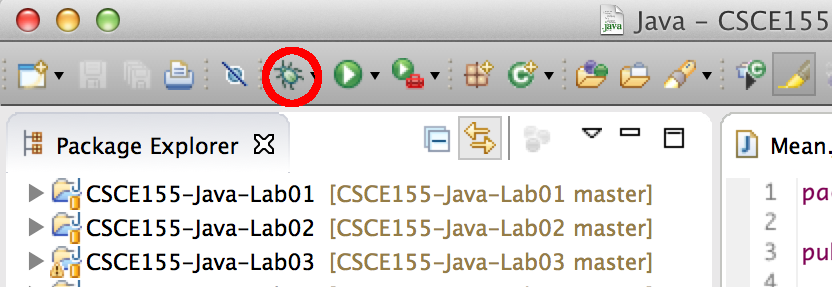
\includegraphics[scale=.75]{eclipseDebugIconMarkUp}
	\end{center}
	Eclipse will prompt you to switch to the Debug Perspective, select yes.
  \item To understand what the problem is; set a breakpoint on line 9 (double click the 
  	left side of the code editor on line 9 until you see the small dot)
  \item Run the program in debug mode: click the ``bug'' next to the play button.  The 
	program will execute until it reaches the breakpoint you set.
	
\begin{figure}[h]
\centering
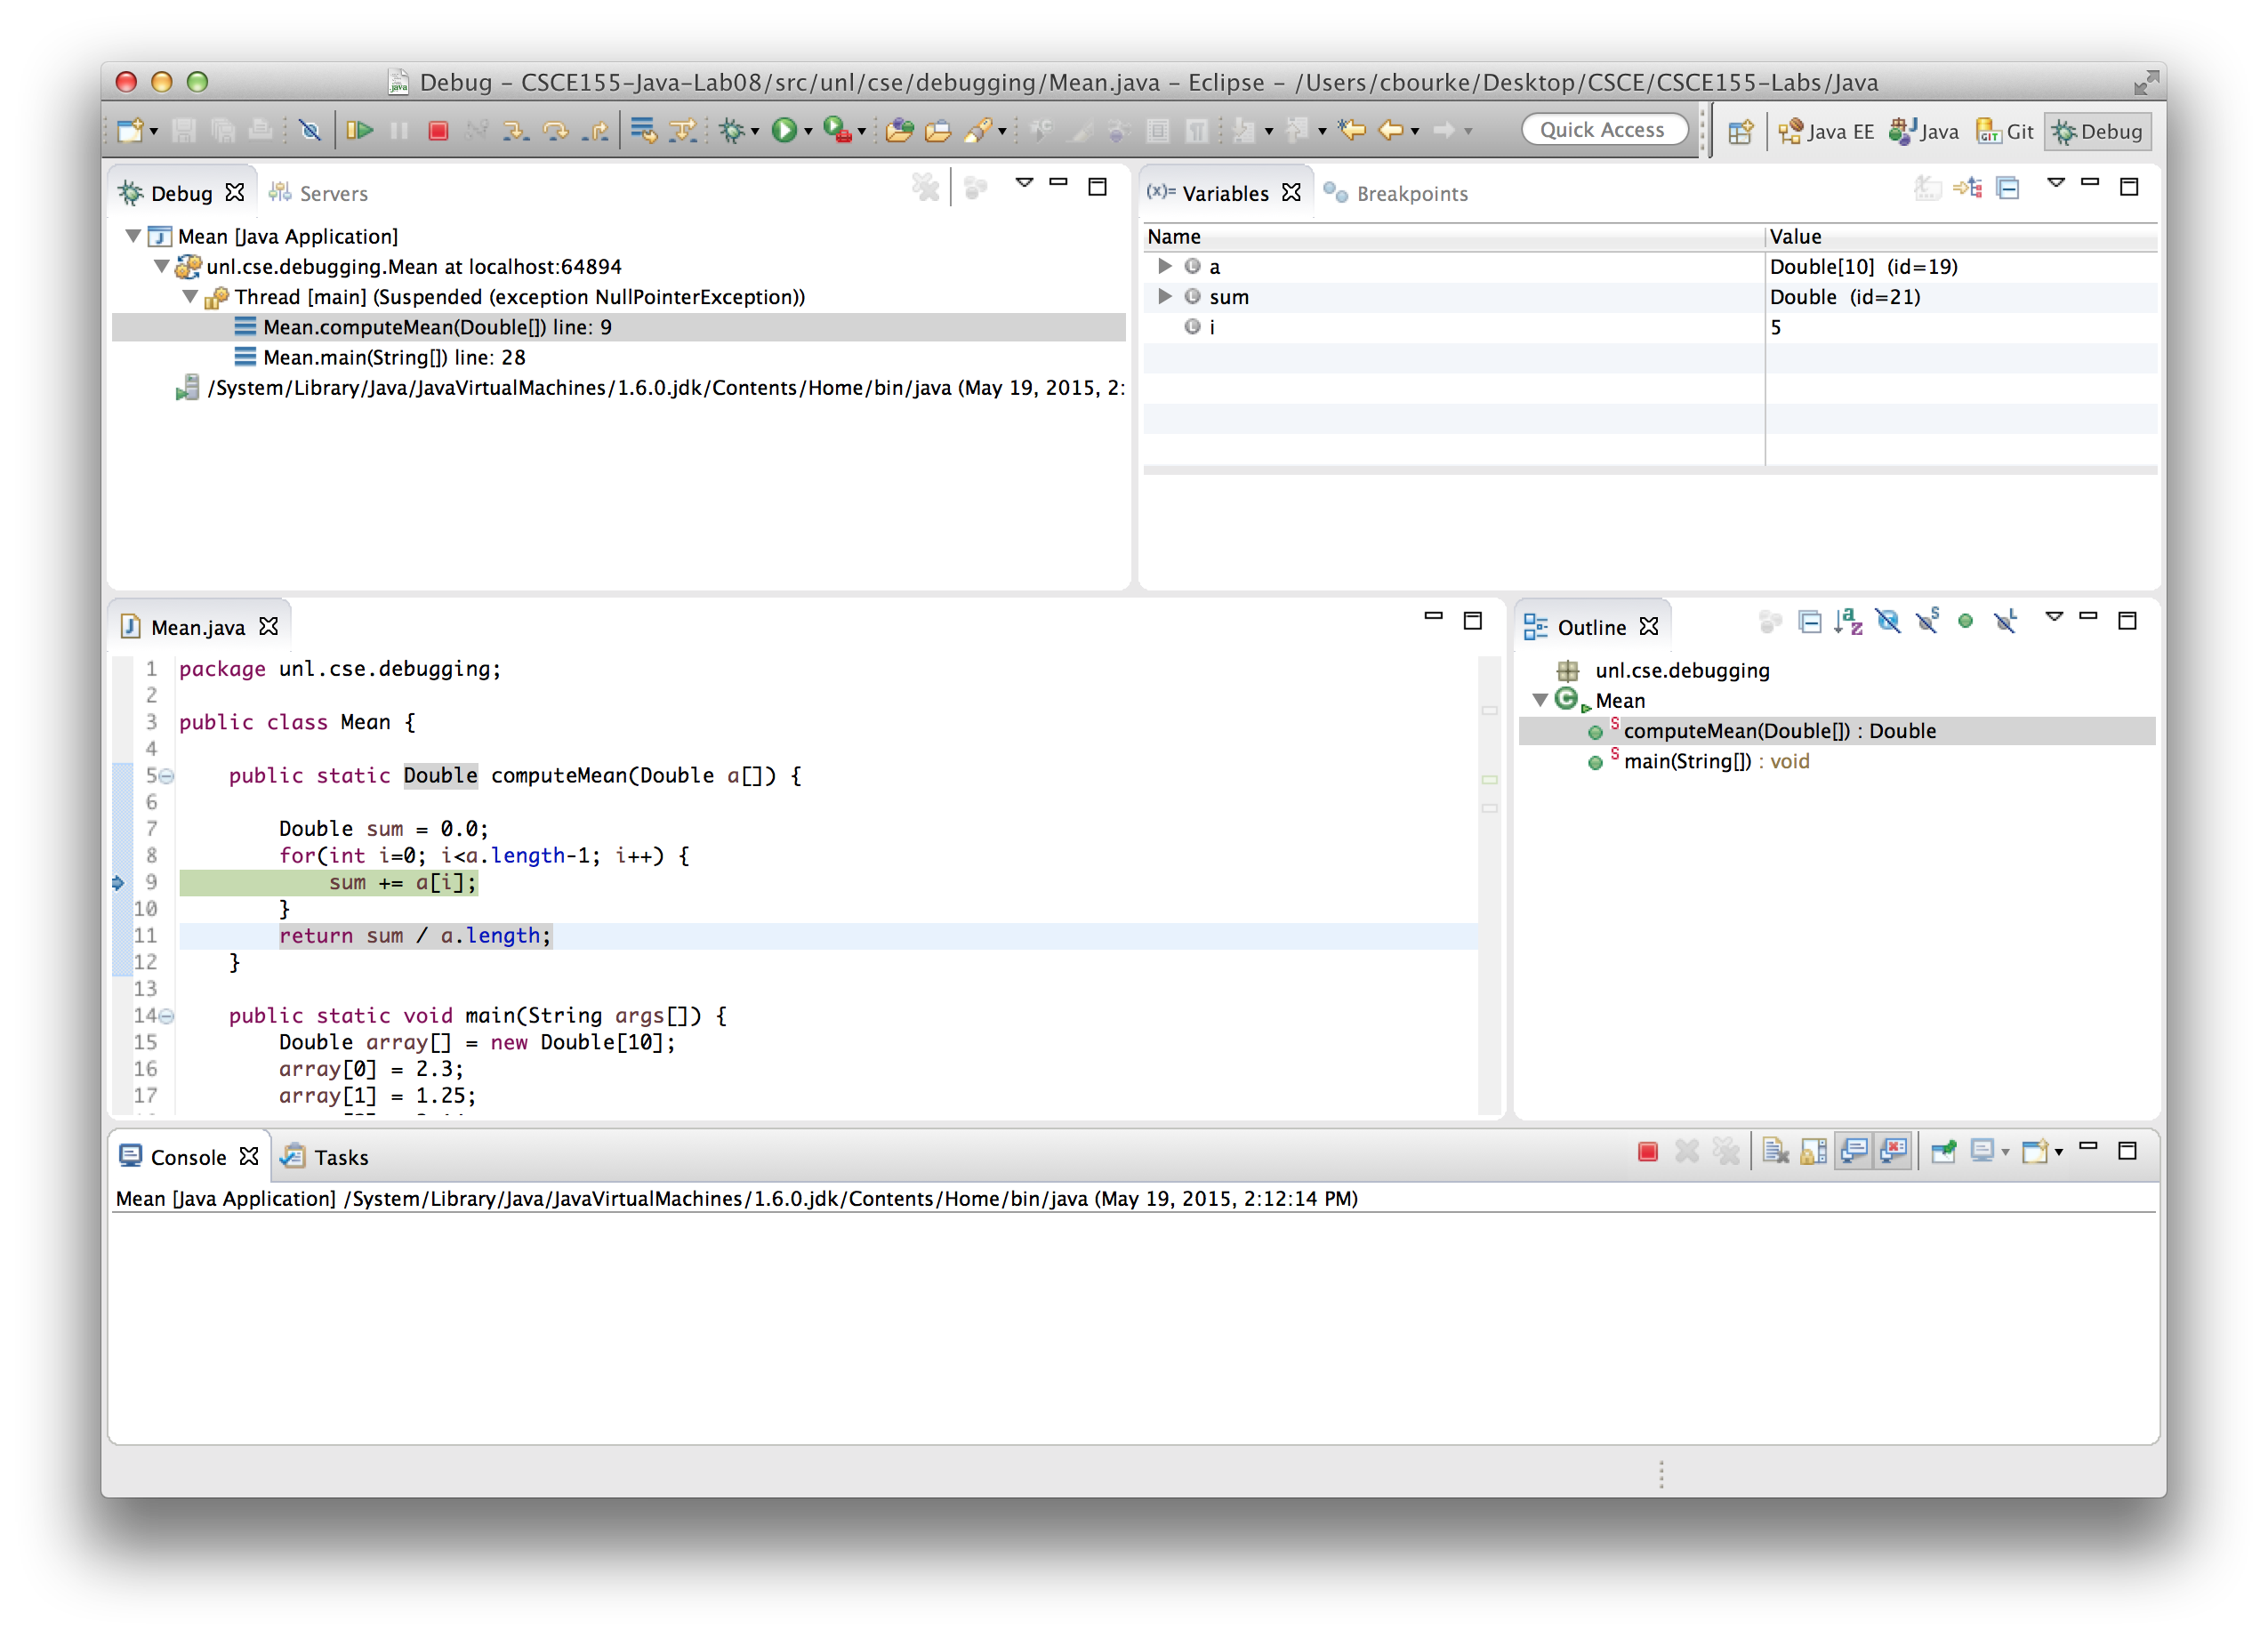
\includegraphics[scale=.35]{eclipseDebugPerspective}
\caption{Eclipse Debug Perspective}
\label{figure:eclipseDebugPerspective}
\end{figure}

  \item Observe the windows (views) and tools (in the toolbar) you have available to you.
	An example screen shot can be found in Figure \ref{figure:eclipseDebugPerspective}.
	\begin{itemize}
	  \item The upper left contains the program's stack (the order of methods that 
	  	have been called so far)
	  \item The upper right contains all local variables and their values; clicking on 
		them also displays their string representation
	  \item The code (and its current line) are displayed at the left
	\end{itemize}
\begin{figure}[h]
\centering
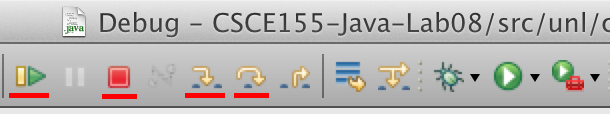
\includegraphics[scale=1.0]{eclipseDebugToolbarMarkUp}
\caption{Eclipse Debug Toolbar}
\label{figure:eclipseDebugToolbar}
\end{figure}
	Debug controls are provided in the toolbar of the program stack window as 
	depicted in Figure \ref{figure:eclipseDebugToolbar}.  As marked in the figure, 
	from left-to-right, each icon does the following:
	\begin{itemize}
	  \item The Play button resumes the program until the next breakpoint
	  \item The Stop button aborts the program execution
	  \item The ``Step into'' arrow steps to the immediate next command
	  \item The ``Step Over'' arrow resumes execution to the end of the next 
		command (so if a method is called it will execute the entire method)
	\end{itemize}	  
  \item Step through the program (click the step over or step into button) and 
  	observe what value the index i takes prior to when an exception is thrown.  
	Deduce what the problem is and fix it.
\end{enumerate}
	

The program still contains a logic error, though it is not apparent.  
\begin{enumerate}
  \item Manually add the values and verify that the answer the program gives 
	is incorrect.
  \item Run the debugger again and step through the entire for-loop.  What 
	value of \mintinline{java}{i} does the loop end on? 
  \item Fix the problem and demonstrate the debugged program to a lab instructor.
\end{enumerate}

The debugger can also be used to detect where a program may get stuck.  
\begin{enumerate}
  \item Change your perspective back to Java (upper right corner)
  \item Drag and drop the TenHellos.java program into the same package as before
  \item Run the program (it is intended to print \mintinline{java}{"Hello!"} ten times) 
	and observe that it does not execute
  \item Kill the program by clicking the ``stop'' button in the console window
  \item Set an appropriate break point to see where the program is getting stuck
  \item Fix the program and demonstrate it to a lab instructor
\end{enumerate}

\section{Advanced Activity (Optional)}

Eclipse like all IDEs can make programming much easier.  Challenge yourself 
by using a command line debugger for Java; specifically jdb.  See the following 
link: (\url{http://docs.oracle.com/javase/1.5.0/docs/tooldocs/windows/jdb.html}) 
and run through this lab again using jdb.

\end{document}
